\documentclass{article}

\usepackage[scale=0.75]{geometry}

% Langues
\usepackage[french]{babel}
\usepackage[utf8]{inputenc}
\usepackage[T1]{fontenc}

% Images
\usepackage{graphicx}
\usepackage{rotating}

% Titre
\title{LaFac.com}
\author{BOSOM - CHAUSSY - DELLOUVE}
%\date{text}

\begin{document}

\maketitle

\vfill
\section*{Introduction}

Afin de travailler la conception de systèmes réels, nous avons créé un modélisé un pseudo-site de vente en ligne.\par
L'implémentation s'est faite en Java et nous devions répondre à plusieurs contraintes, à savoir un système de gestion de personnes, de produits et de différentes offres applicables.
\vfill

\newpage

\section*{Conception}

\subsection*{Diagramme de classe}


\begin{sidewaysfigure}[ht]
	\vfill\hfill % Centrage sur la page
	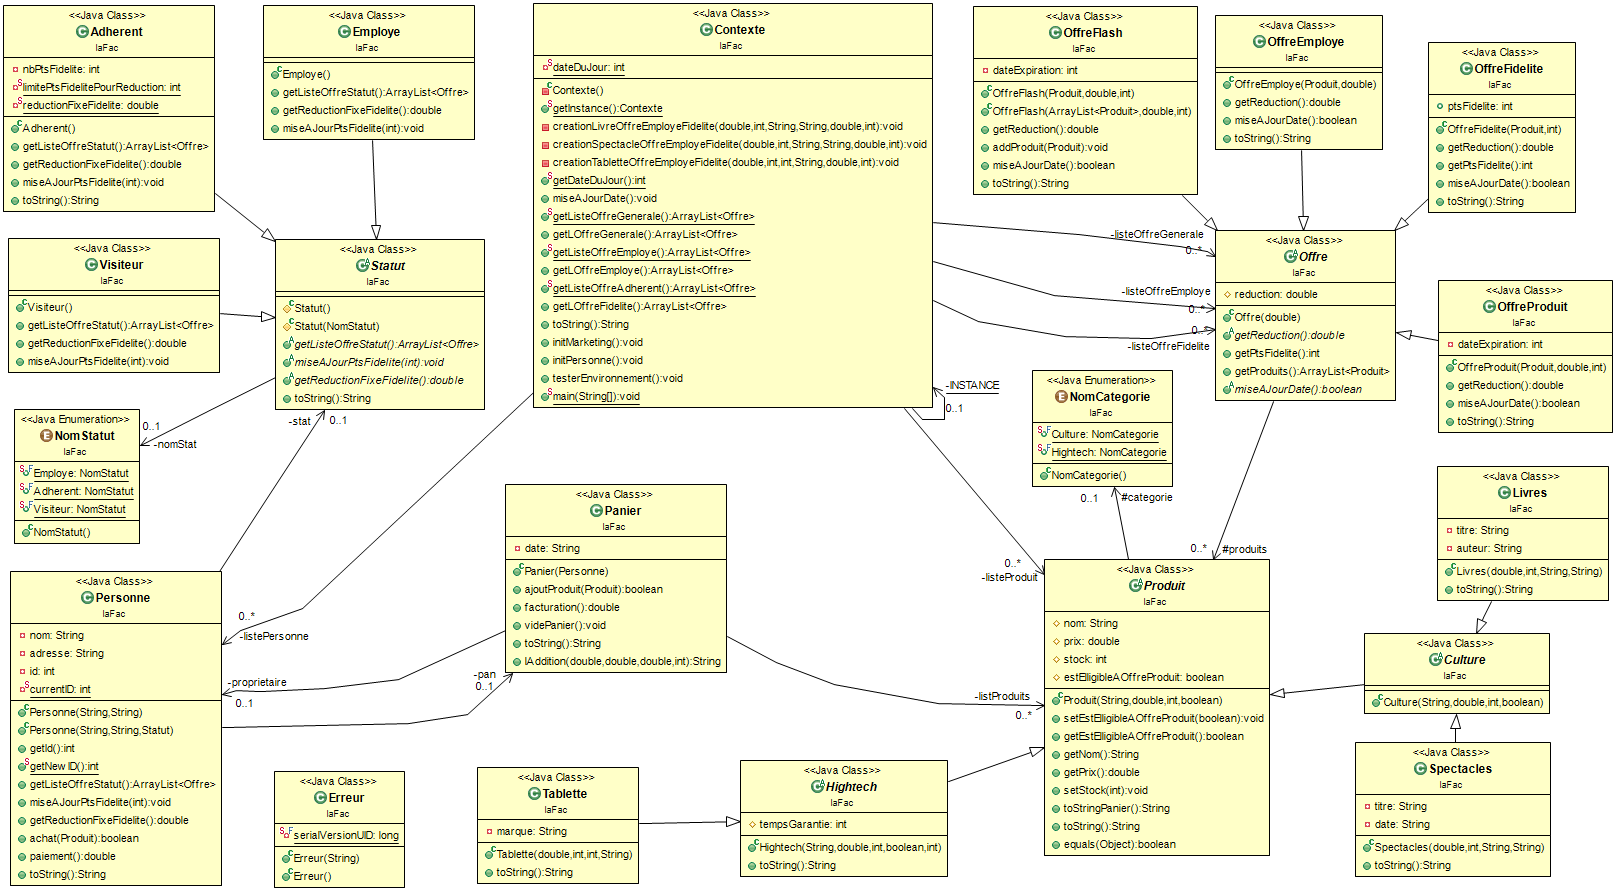
\includegraphics[scale=0.36]{diagUML.png}
	\hfill\vfill % Centrage sur la page
	\caption{Diagramme de classe}
\end{sidewaysfigure}

\subsection*{Diagrammes de séquences}

\clearpage % Force l'affichage des images flottantes avant de passer une page

\vfill
\section*{Conclusion}

Ce projet nous a permis de réfléchir à un problème concret, mettant en œuvre les connaissances acquises durant le cours.\par
Nous avons utilisé plusieurs design pattern, afin de répondre aux différentes contraintes du sujet,
et la généricité du langage afin que les interactions entre les objets soient le plus simple et le plus clair possible, tout en offrant une possibilité d'évolution du code.\par
En résumé, il s'agissait d'un exercice enrichissant qui nous aura permis d'acquérir de nouvelles connaissances.
\vfill


\end{document}